\documentclass[11pt, oneside]{article}   	% use "amsart" instead of "article" for AMSLaTeX format
\usepackage{geometry}                		% See geometry.pdf to learn the layout options. There are lots.
\geometry{letterpaper}                   		% ... or a4paper or a5paper or ... 
\usepackage{graphicx}				% Use pdf, png, jpg, or eps§ with pdflatex; use eps in DVI mode
								% TeX will automatically convert eps --> pdf in pdflatex		
\usepackage{amssymb}
\usepackage{amsmath}
\usepackage{parskip}
\usepackage{color}
\usepackage{hyperref}

\graphicspath{{/Users/telliott_admin/Dropbox/Tex/png/}}
% \begin{center} 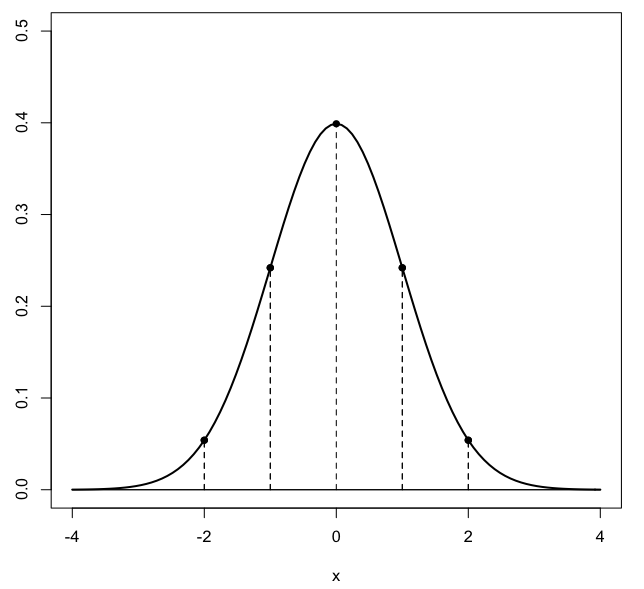
\includegraphics [scale=0.4] {gauss3.png} \end{center}

%break
\title{Spherical cap}
\date{}

\begin{document}
\maketitle
\Large


Here is a figure from Wolfram for a spherical cap.  We are interested in formulas for the area and volume of the solid obtained by slicing through a sphere, where the height of the cap that is produced is $h$, and the distance of closest approach to the center of the sphere is $R-h$.
\begin{center} 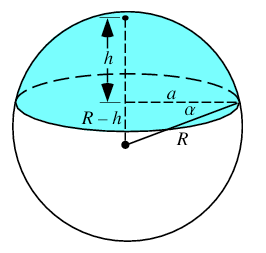
\includegraphics [scale=0.6] {spherical_cap.png} \end{center}

\subsection*{geometry}
If we start from the equator, and think about a thin belt going around the sphere, the belt has length equal to the circumference $2\pi R$ and width $h$, and thus area $S$:
\[ S = 2 \pi R h \]

We believe this should be the formula for the surface area of a belt of width $h$, at least near the equator.  In the figure, this width is labeled as $R-h$, because we are more interested in the cap.  Thus, for the calculation below, this area will be $2\pi R(R-h)$.

Consider that the total surface area of the hemisphere is $2\pi R^2$ so the area of the cap is the difference
\[ S = 2\pi R^2 -  2 \pi R (R-h) = 2 \pi Rh \]

That's a surprising result, that the area of the cap depends only on $R$ and its width (here called $h$).  At least, that is certainly true in the limit as the width of the belt at the equator is very small.

\subsection*{polar cap}
Furthermore, if we look in the figure at the right triangle with $h$ and $a$ as the sides, we can draw the hypotenuse of that triangle and call it $r$ (it's not actually labeled in the figure).  
\begin{center} 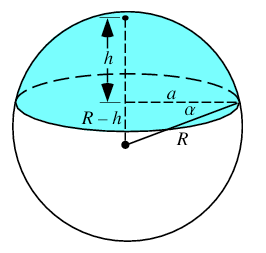
\includegraphics [scale=0.6] {spherical_cap.png} \end{center}

It is sometimes called the slant height.  We calculate
\[ a^2 = R^2 - (R - h)^2 = 2 Rh - h^2 \]
\[ r^2 = a^2 + h^2 = 2 Rh - h^2 + h^2 = 2 Rh \]

Now think about a very small spherical cap, then it would be almost flat, a circle, and its radius would be $r$ and area
\[ S = \pi r^2 \]
But $r^2 = 2Rh$, so again we have the same formula for the surface area of a small cap and a belt near the equator!

\subsection*{General case}
Consider a belt of width $h$ at a position somewhere in the temperate latitudes of the sphere, not close to either the pole or the equator.

We use a thin belt, so that going north toward the pole the surface of the sphere is approximately flat.  As before, $h$ is the width of the projection of the belt on the $z$-axis.  

The width $w$ of the belt on the surface is larger than $h$, because $w$ is not vertical but tilted toward the $z$-axis.  And since the surface is flat, this angle with the $z$-axis is constant over the width of the belt.

Draw a ray from the center of the sphere to the point where the belt is. The ray makes an angle $s$ with the $xy$-plane, at the center of the sphere.  The radius $a$ at the position of the belt is smaller than $R$ by a factor of $\cos s$. 
\[ a = R \cos s \]
\begin{center} 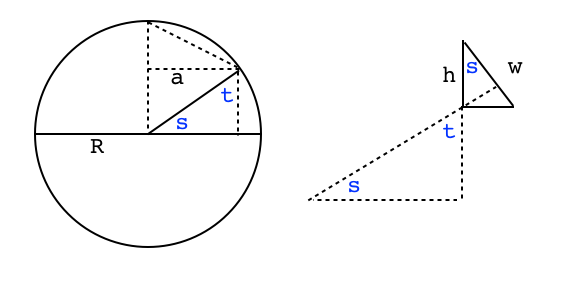
\includegraphics [scale=0.6] {sphcap2.png} \end{center}
The tangent to the sphere at this point (namely, $w$) is perpendicular to the ray.  In the right panel, we see a small triangle on the surface of the sphere with sides $w$ and $h$.

All three of the triangles shown in the right panel are right triangles, with complementary angles $s$ and $t$ (not all of them are labeled).  Can you see that the angle between $h$ and $w$ is $s$?

Therefore, the slant height $w$ of the belt is larger than $h$ by the factor of $\cos s$.
\[ h = w \cos s \]
So the true area is
\[ 2 \pi \ a \ w = 2 \pi R \cos s \frac{h}{\cos s} = 2 \pi R h \]
The cosine of the angle comes in twice, and these factors cancel.  

The formula $2\pi R h$ is correct everywhere.
\subsection*{calculus}
We imagine rotating a semi-circle around the $x$-axis to form a volume of revolution.  As we've seen in a previous chapter
\[ S = \int 2 \pi y \ \sqrt{1 + (\frac{dy}{dx})^2} \ dx \]
The square root comes from the surface area element.  This formula looks unwieldy (and often it is).  But in this particular case it simplifies dramatically.

If we take a circle as the curve, with formula
\[ x^2 + y^2 = R^2 \]
\[ 2x \ dx + 2y \ dy = 0 \]
\[ \frac{dy}{dx} = - \frac{x}{y} \]
So
\[ S = 2 \pi \int y \ \sqrt{1 + \frac{x^2}{y^2}} \ dx \]
\[ S = 2 \pi \int \sqrt{y^2 + x^2} \ dx \]
\[ S = 2 \pi \int R \ dx = 2 \pi R x \]
Evaluated between $x=a \to x=b$
\[ s = 2 \pi R (b-a) = 2 \pi R h \]

This makes it very clear that the area does not depend where we are on the sphere.  A spherical cap with height $h$ has the same area as a belt of width $h$ wrapped around the equator, or any belt of width $h$ in between the two.

And as we noticed before, the area of a belt or sperical cap, $2 \pi R h$, is equal to the surface area of a cylinder of radius $R$ and height $h$, the so-called hat-box theorem of Archimedes.
\begin{center} 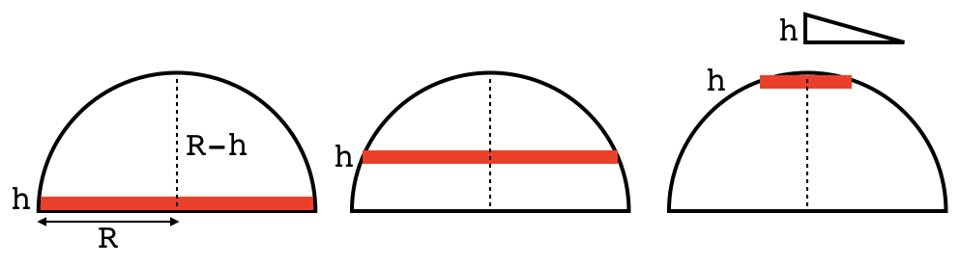
\includegraphics [scale=0.4] {hatbox.jpg} \end{center}

\section*{spherical cap:  volume}
\subsection*{calculus}
Here we will derive the formula for the volume of a spherical cap.  This is the solid obtained by slicing off a part of a sphere with a plane. 
\begin{center} 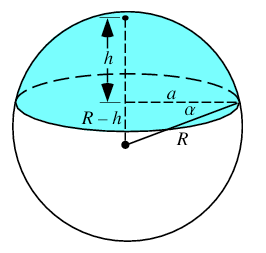
\includegraphics [scale=0.6] {spherical_cap.png} \end{center}
The formula is 
\[ V_{cap} = \frac{1}{3} \pi h^2(3R - h) \]
or equivalently
\[ V = \pi(Rh^2 - \frac{1}{3} h^3 )\]
We can see that this equation makes sense for the extreme case where $h=R$.  We get 

\[ V = \frac{1}{3} \pi R^2(3R - R) =   \frac{2}{3} \pi R^3 \]

One way to do spherical volumes is by integration of slices as shown in this figure (from Strang)
\begin{center} 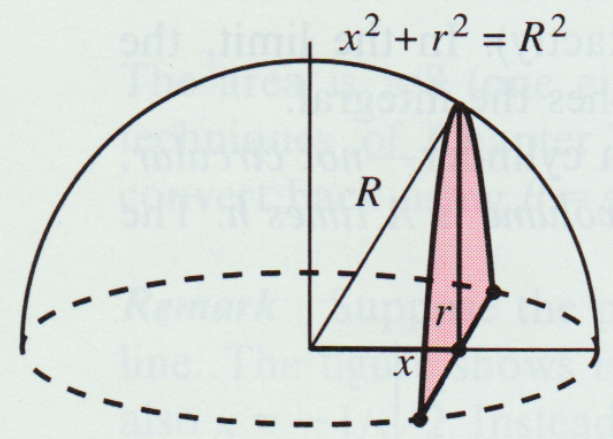
\includegraphics [scale=0.4] {sph_slices2.png} \end{center}

This approach is basically the same as what I showed when we calculated the volume of the sphere using calculus, before.

In Strang's derivation, at each value of $x$, the hemisphere (of radius $R$) has a cross-section that is a half-circle with radius $r$ such that
\[ x^2 + r^2 = R^2 \]
the area of this hemisphere cross-section is
\[ A = \frac{1}{2} \pi r^2= \frac{1}{2} \pi (R^2 - x^2) \]
For the whole sphere, each cross-section is a circle with area
\[ A =  \pi r^2= \pi (R^2 - x^2) \]

For the volume, we just add up all these slices.  To make it simple, take $x$ from $0 \to R$ 
\[ V =  \pi \int_{0}^{R}  (R^2 - x^2) \ dx \]
\[ =  \pi \ [ \ R^2x - \frac{1}{3}x^3 \ ] \ \bigg |_{0}^R =  \frac{2}{3}\pi R^3 \]
Multiply by a factor of $2$ to get the whole thing.

The key insight is, we can get a spherical cap (or a belt), just by changing the lower limit of integration to $x=R-h$  !!  
\begin{center} 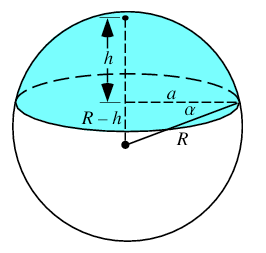
\includegraphics [scale=0.6] {spherical_cap.png} \end{center}
We need to evaluate
\[ V = \pi \ [ \ R^2x - \frac{1}{3}x^3 \ ] \ \bigg |_{R-h}^R \]
Leave aside the factor of $\pi$, and break the expression into two parts 
\[ R^2x  \ \bigg |_{R-h}^R - \frac{1}{3} x^3  \ \bigg |_{R-h}^R \]
For the left term we get
\[ R^3 - R^3 + R^2h = R^2h\]
For the right side we get
\[ -\frac{1}{3} R^3 + \frac{1}{3}(R-h)^3 ) \]
\[=  -\frac{1}{3} R^3 + \frac{1}{3} R^3 - R^2h + Rh^2 -\frac{1}{3} h^3 \]
Adding left and right terms together, the $R^2h$ terms cancel, and we have finally
\[ V = \pi (Rh^2 - \frac{1}{3} h^3) \]
Factoring out $h^2/3$
\[ V = \frac{1}{3} \pi h^2 (3R -h) \]
which is the formula we gave at the top.

We can calculate the volume of \emph{any} spherical belt by using the appropriate limits of integration.  For example, the belt from $r=0 \rightarrow r = R-h$ has volume
\[ V = \pi \ [ \ R^2x - \frac{1}{3}x^3 \ ] \ \bigg |_{0}^{R-h} \]
Leaving the $\pi$ aside for now
\[ R^2(R-h) - \frac{1}{3}(R-h)^3 \]
\[ R^3 - R^2h - \frac{1}{3}(R^3 - 3R^2h + 3Rh^2 - h^3) \]
\[ \frac{2}{3}R^3 - Rh^2 + \frac{1}{3} h^3  \]
With the factor of $\pi$
\[ V = \pi ( \frac{2}{3}R^3 - Rh^2 + \frac{1}{3} h^3 )  \]
Adding the cap and the belt together:
\[ V_{tot} =  \pi( Rh^2 - \frac{1}{3}h^3 + \frac{2}{3}R^3 - Rh^2 + \frac{1}{3} h^3) \]
Almost everything cancels
\[ V_{tot} =  \pi( \frac{2}{3}R^3) \]
The cap and the belt together make up a hemisphere.



\end{document}